\documentclass{oblivoir}
\usepackage{amsmath,amssymb,amsthm,kotex,mdframed,paralist,kswrapfig}

\newcounter{num}
\newcommand{\prob}
{\bigskip\noindent\refstepcounter{num}\textbf{문제 \arabic{num})}\par}

\newcommand{\subprob}
{\bigskip\noindent\textbf{추가문제 \arabic{num}-1)}\par}

\newcommand{\subprobb}
{\bigskip\noindent\textbf{추가문제 \arabic{num}-2)}\par}

\newcommand{\ans}{{\raggedleft\textbf{답 : (\qquad\qquad\qquad\qquad\qquad\qquad)}
\par}\bigskip\bigskip}


\newcommand\ga{\text{(가)}}
\renewcommand\na{\text{(나)}}


%%%
\begin{document}
\Large

\title{승재 15 - 6학년 2학기 - 08}
\author{}
\date{\today}
\maketitle
%\tableofcontents

\newpage


%
\prob
다음 \(\square\)에 들어갈 알맞은 숫자를 쓰세요.

\begin{enumerate}[(1)]
\item
\(4:1=\square:\frac37\)
\item
\(3:\frac25=7:\square\)
\item
\(\frac23:\frac32=4:\square\)
\item
\(\frac25:2=3:\square\)
\item
\(1:\frac43=\frac23:\square\)
\item
\(\frac53:\frac52=\square:10\)
\item
\(\frac{10}3:\frac{15}2=\square:\frac{25}2\)
\item
\(\frac{15}7:\frac{12}{11}=\square:56\)
\item
\(\frac{11}5:132=\square:4\)
\item
\(\frac{36}7:5=\frac{12}7:\square\)
\item
\(1.69:1.43=\square:22\)
\item
\(300:750=27:\square\)
\item
\(40:125=0.16:\square\)
\end{enumerate}

\newpage

%
\prob
준호가 이번 시험에서 받은 국어, 영어, 수학 점수를 살펴보았더니, 국어 점수는 영어 점수의 \(\frac{25}{27}\)이고 수학 점수는 국어 점수의 \(\frac{16}{15}\)이었습니다.
이 때, 수학 점수:영어 점수를 가장 간단한 자연수의 비로 나타내고, 그 풀이과정을 쓰세요.

\begin{mdframed}
\textbf{풀이 : }
\vspace{0.2\textheight}
\end{mdframed}
\ans

%
\prob
상재의 영어 점수는 국어 점수의 1.25이고 수학 점수는 영어 점수의 0.96입니다.
이 때, 수학 점수:국어 점수를 가장 간단한 자연수의 비로 나타내고, 그 풀이과정을 쓰세요.

\begin{mdframed}
\textbf{풀이 : }
\vspace{0.2\textheight}
\end{mdframed}
\ans

\newpage

%
\prob
선분 AB와 선분 BC의 길이의 비는 1:6이고 선분 BC와 선분 CD의 길이의 비는 3:2입니다.
이때 다음 물음에 답하세요.
\begin{figure}[h!]
\centering
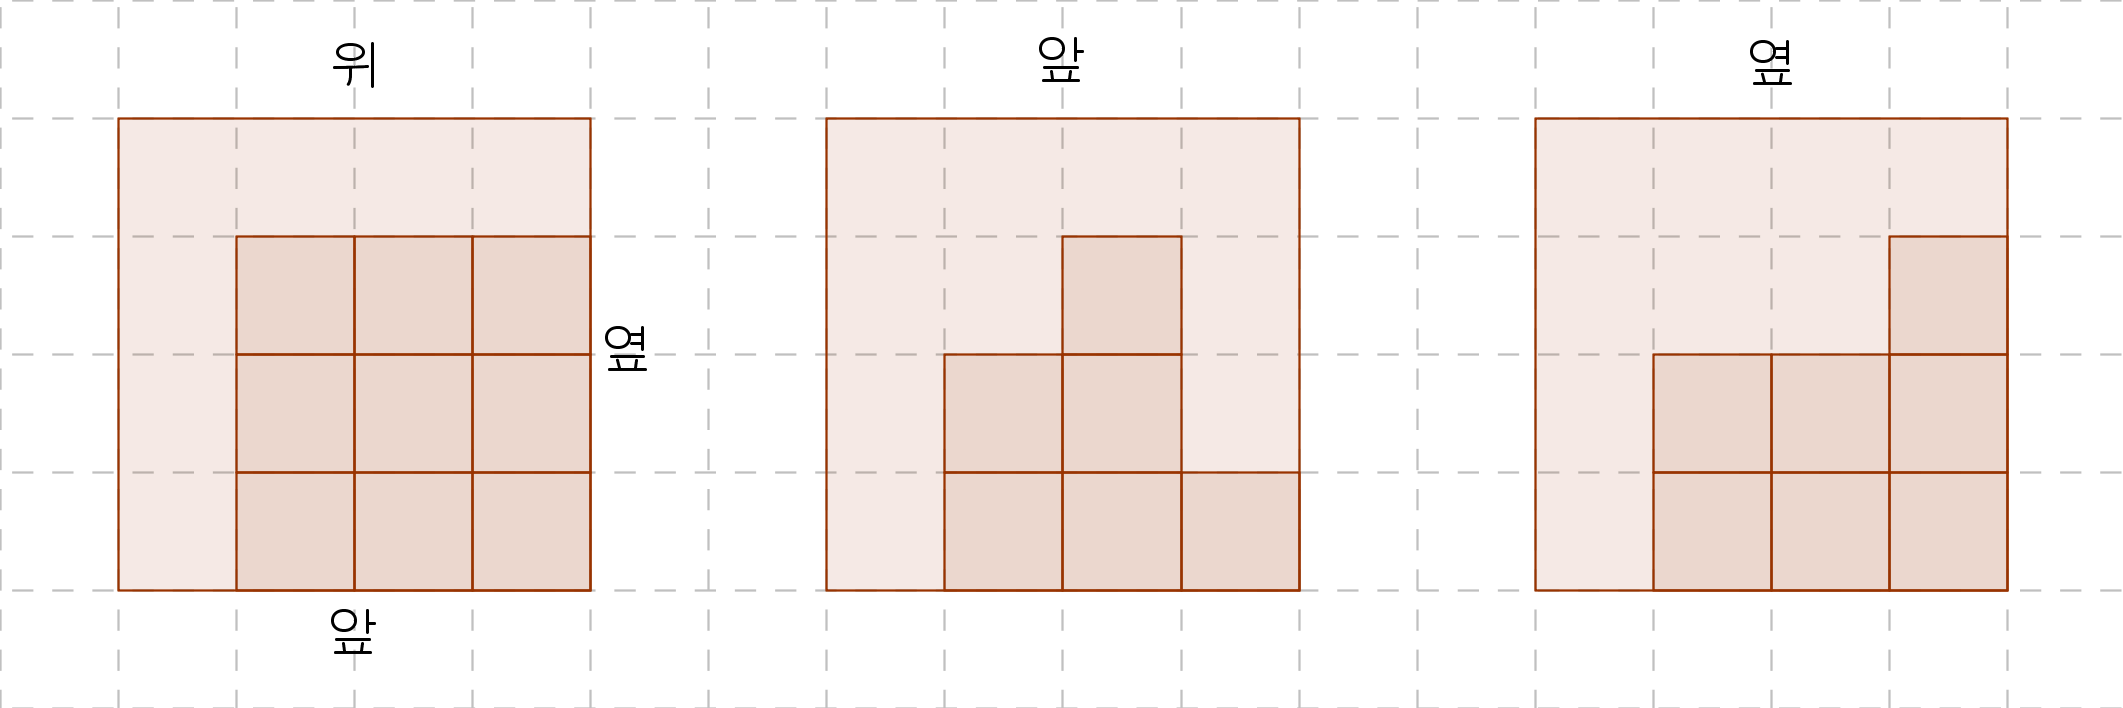
\includegraphics[width=0.9\textwidth]{04}
\end{figure}

(1) 선분 AB와 선분 CD의 길이의 비를 구하세요.

\ans

(2) 선분 AB와 선분 BD의 길이의 비를 구하세요.

\ans

(3) 선분 AB, 선분 BC, 선분 CD의 길이의 비를 구하세요.

\ans

%
\prob
선분 AB와 선분 BC의 길이의 비는 4:1이고 선분 BC와 선분 CD의 길이의 비는 2:5입니다.
이때 다음 물음에 답하세요.
\begin{figure}[h!]
\centering
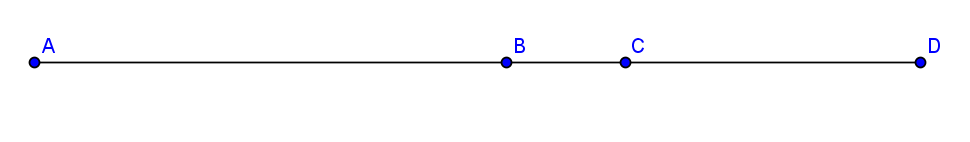
\includegraphics[width=0.9\textwidth]{05}
\end{figure}

(1) 선분 AB와 선분 CD의 길이의 비를 구하세요.

\ans

(2) 선분 AB, 선분 BC, 선분 CD의 길이의 비를 구하세요.

\ans

%
\prob
선분 AB와 선분 BC의 길이의 비는 1:3이고 선분 BC와 선분 BD의 길이의 비는 2:3입니다.
이때 다음 물음에 답하세요.
\begin{figure}[h!]
\centering
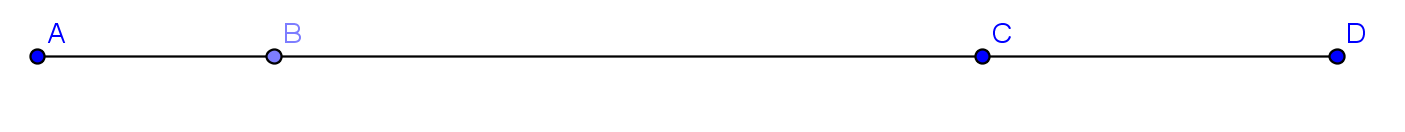
\includegraphics[width=0.9\textwidth]{06}
\end{figure}

(1) 선분 BC와 선분 CD의 길이의 비를 구하세요.

\ans

(2) 선분 AB, 선분 BC, 선분 CD의 길이의 비를 구하세요.

\ans

%
\prob
선분 AB와 선분 AD의 길이의 비는 2:5이고 선분 AD와 선분 CD의 길이의 비는 3:1입니다.
이때 다음 물음에 답하세요.
\begin{figure}[h!]
\centering
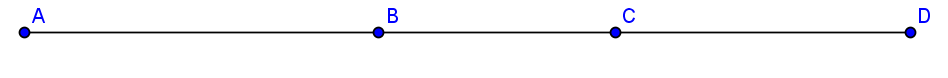
\includegraphics[width=0.9\textwidth]{07}
\end{figure}

(1) 선분 AB와 선분 BD의 길이의 비를 구하세요.

\ans

(1) 선분 AC와 선분 CD의 길이의 비를 구하세요.

\ans

(3) 선분 AB, 선분 BC, 선분 CD의 길이의 비를 구하세요.

\ans

\newpage
%
\prob
같은 크기의 옆면으로 만든 서로 다른 원기둥의 부피를 구하려고 합니다.
물음에 답하세오.
(원주율:3.1)
\begin{figure}[h!]
\centering
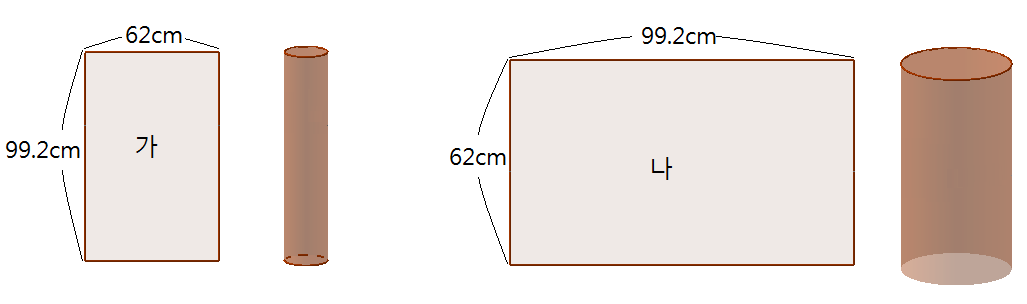
\includegraphics[width=0.9\textwidth]{08}
\end{figure}

(1) 직사각형 `가'를 옆면으로 하여 만든 원기둥의 부피는 몇 cm\(^3\) 입니까?

\ans

(2) 직사각형 `나'를 옆면으로 하여 만든 원기둥의 부피는 몇 cm\(^3\) 입니까?

\ans


\newpage
%
\prob
같은 크기의 옆면으로 만든 서로 다른 원기둥의 부피를 구하려고 합니다.
물음에 답하세오.
(원주율:3.1)
\begin{figure}[h!]
\centering
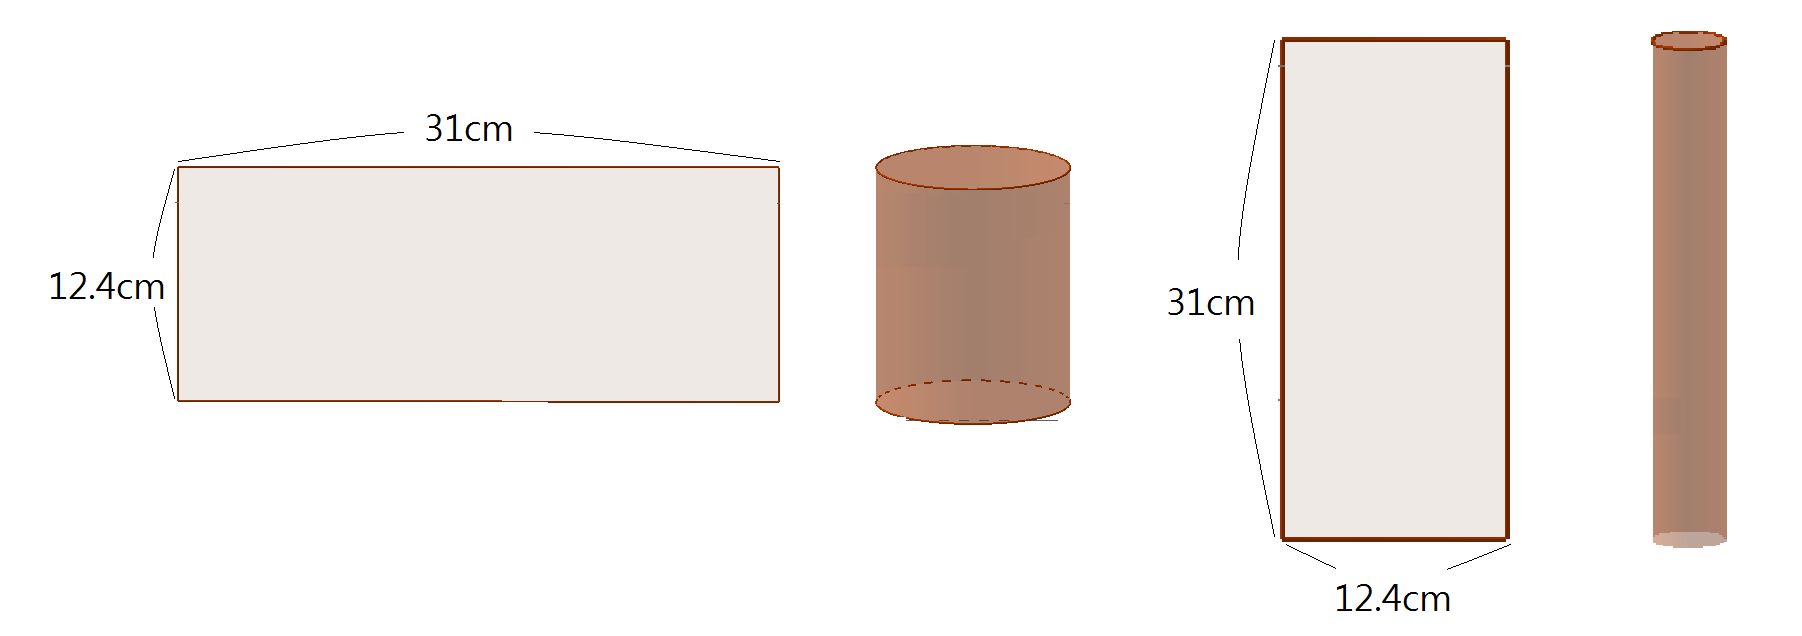
\includegraphics[width=0.9\textwidth]{09}
\end{figure}

(1) 직사각형 `가'를 옆면으로 하여 만든 원기둥의 부피는 몇 cm\(^3\) 입니까?

\ans

(2) 직사각형 `나'를 옆면으로 하여 만든 원기둥의 부피는 몇 cm\(^3\) 입니까?

\ans

\newpage
\prob
입체도형의 겉넓이는 몇 cm\(^2\)입니까?
(원주율:3.14)

\begin{figure}[h!]
\centering
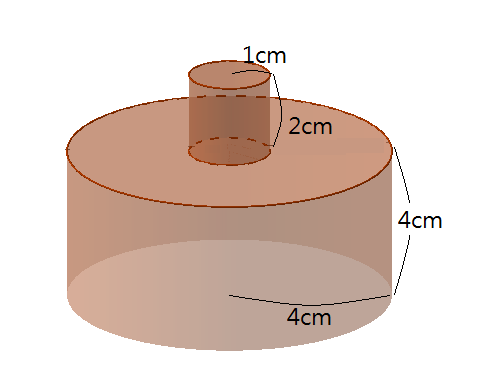
\includegraphics[width=0.9\textwidth]{10}
\end{figure}

\newpage
\prob
입체도형의 겉넓이는 몇 cm\(^2\)입니까?
(원주율:3.14)

\begin{figure}[h!]
\centering
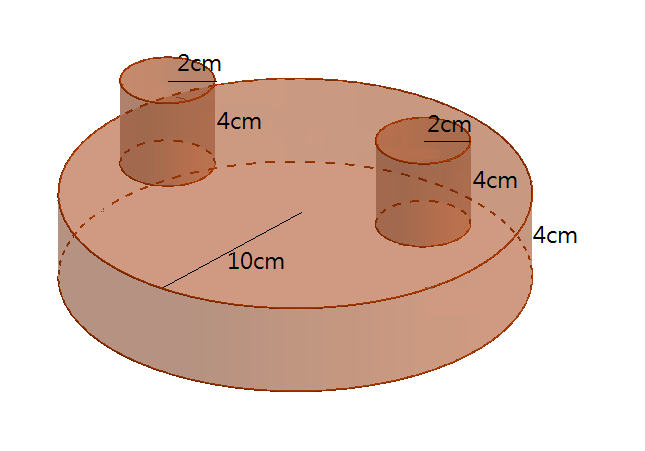
\includegraphics[width=0.9\textwidth]{11}
\end{figure}

\newpage
\prob
다음 그림에서 선분 BH의 길이를 구하세요.
\begin{figure}[h!]
\centering
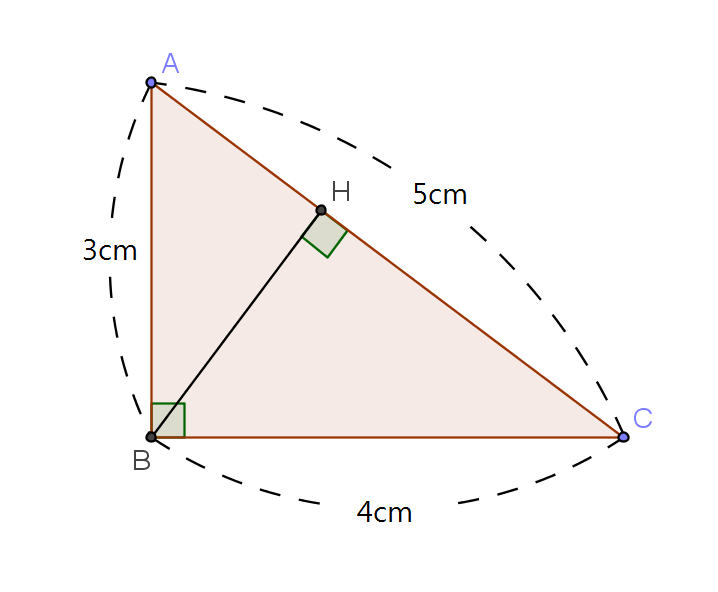
\includegraphics[width=0.7\textwidth]{12}
\end{figure}

\ans

\newpage
\prob
다음 그림에서 선분 AC의 길이를 구하세요.
(선분 DH는 \(\frac{60}{13}\)cm입니다.)
\begin{figure}[h!]
\centering
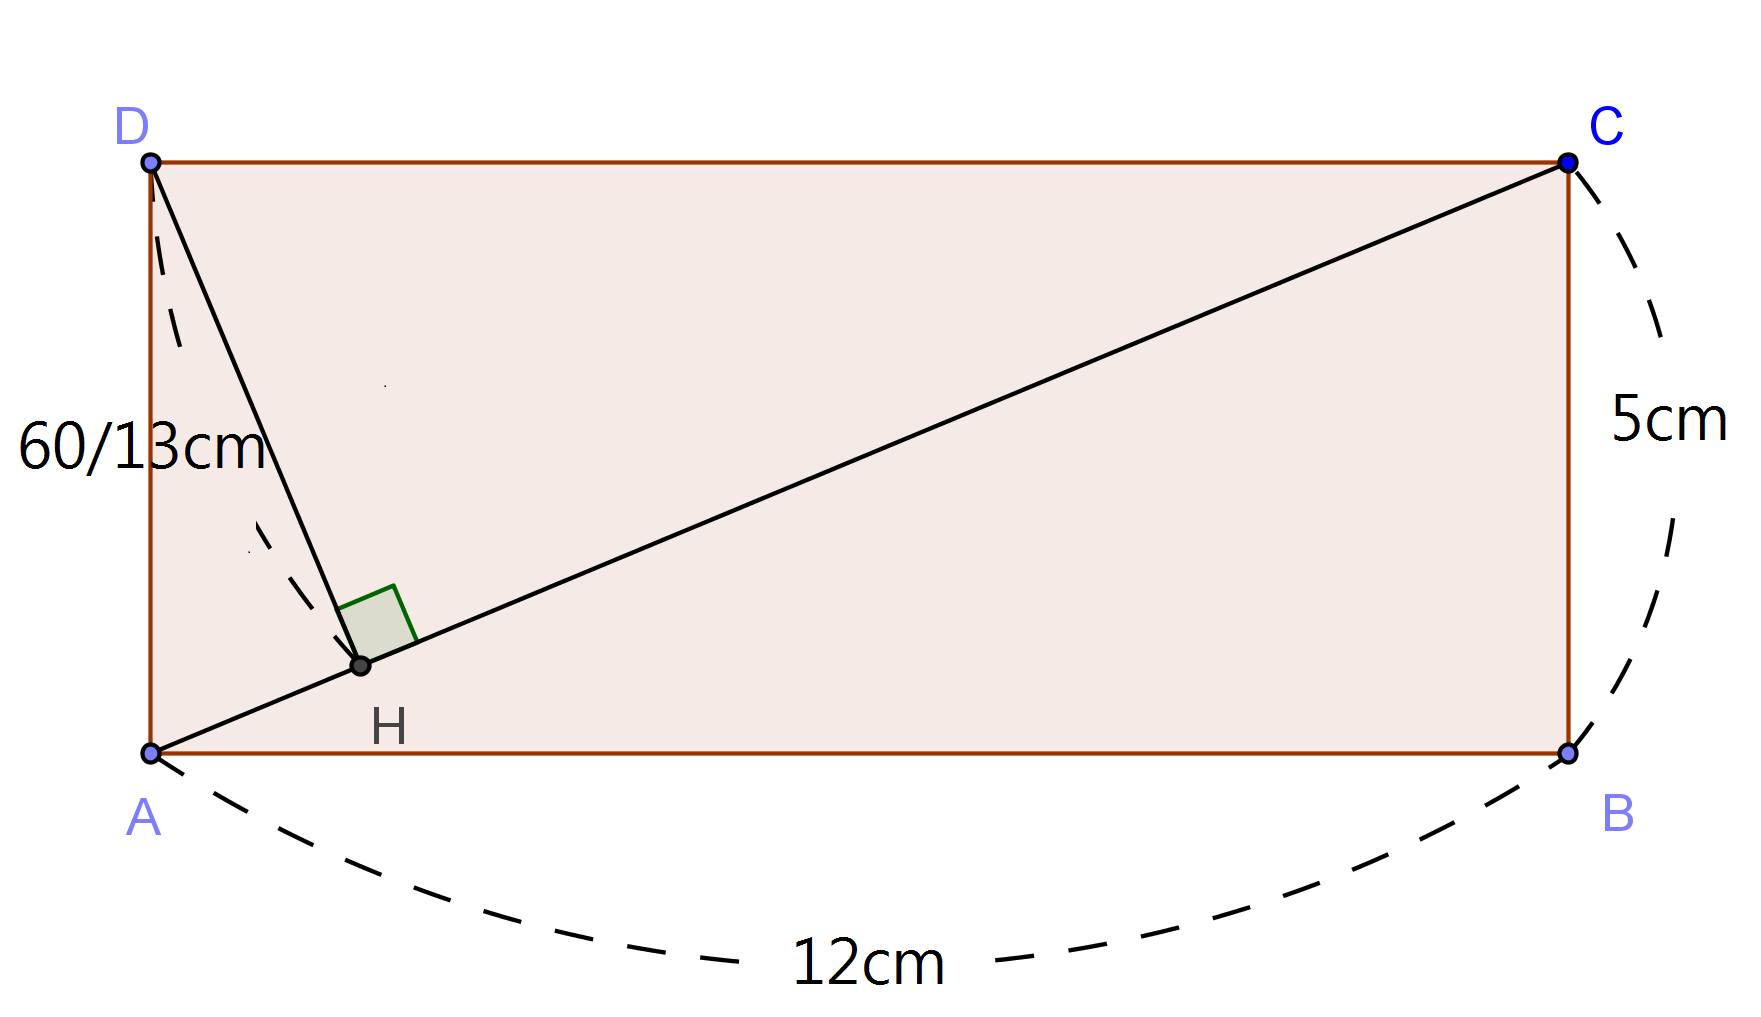
\includegraphics[width=0.7\textwidth]{13}
\end{figure}

\ans

\end{document}